\section{Implementation}

To realize our PGLAS, we have implemented a parallel distributed key/value store, 
PDHT. A novel aspect of this system is its implementation directly on top of the
Portals4 network interface~\cite{portals4}. The Portals framework provides several low-level 
data abstractions that map nicely onto the PGLAS operations supported by PDHT.

PDHT adopts a one-sided communication model which operates with PGAS-like
semantics, providing put, get, and atomic operations. By implementing PDHT directly
with the Portals interface, we can take advantage of message-passing features
that permit an efficient, hardware-offload friendly version of a PGLAS.
Describing some of the primary abstractions with the Portals network model is
helpful to better understand the PDHT implementation.

\subsection{Portals Networking Interface}

% provides several low-level adts for pdht
% one-sided, try to avoid involving processor on the target node
% matching is for MPI, novel application to matching interface
% abstractions for implementing PDHT
% using portals allows us to be hardware offload friendly as compared to 
% traditional PGAS techniques.

The Portals interface provides low-level data abstractions that can be used to
implement both PGAS and message-passing run-times. PDHT relies on a one-sided
communication model that aims to avoid processor involvement on the target
node. Portals supports messaging via a {\em matching interface} model intended to
support MPI (i.e. two-sided matched send/receive pairs). It also provides a
lightweight {\em non-matching} interface that is intended to support one-sided
communications without the need for the matching and ordering semantics
required by MPI. Our implementation uses a novel application of the Portals
matching interface to provide a one-sided model that is the basis of the PDHT
PGLAS. 

The Portals matching interface was designed to support systems that provide a
two-sided messaging model with guarantees about message ordering. The
implementation strategy that underlies PDHT is to separate these two concerns.
PDHT utilizes the matching interface operations to fulfill put and get
operations but makes no guarantees about the interleaving of requests. We
review the primary concepts in the Portals interface to provide clarity for
discussing the implementation of PDHT.


% use figure* to span both cols
\begin{figure}[ht]
  \centering
  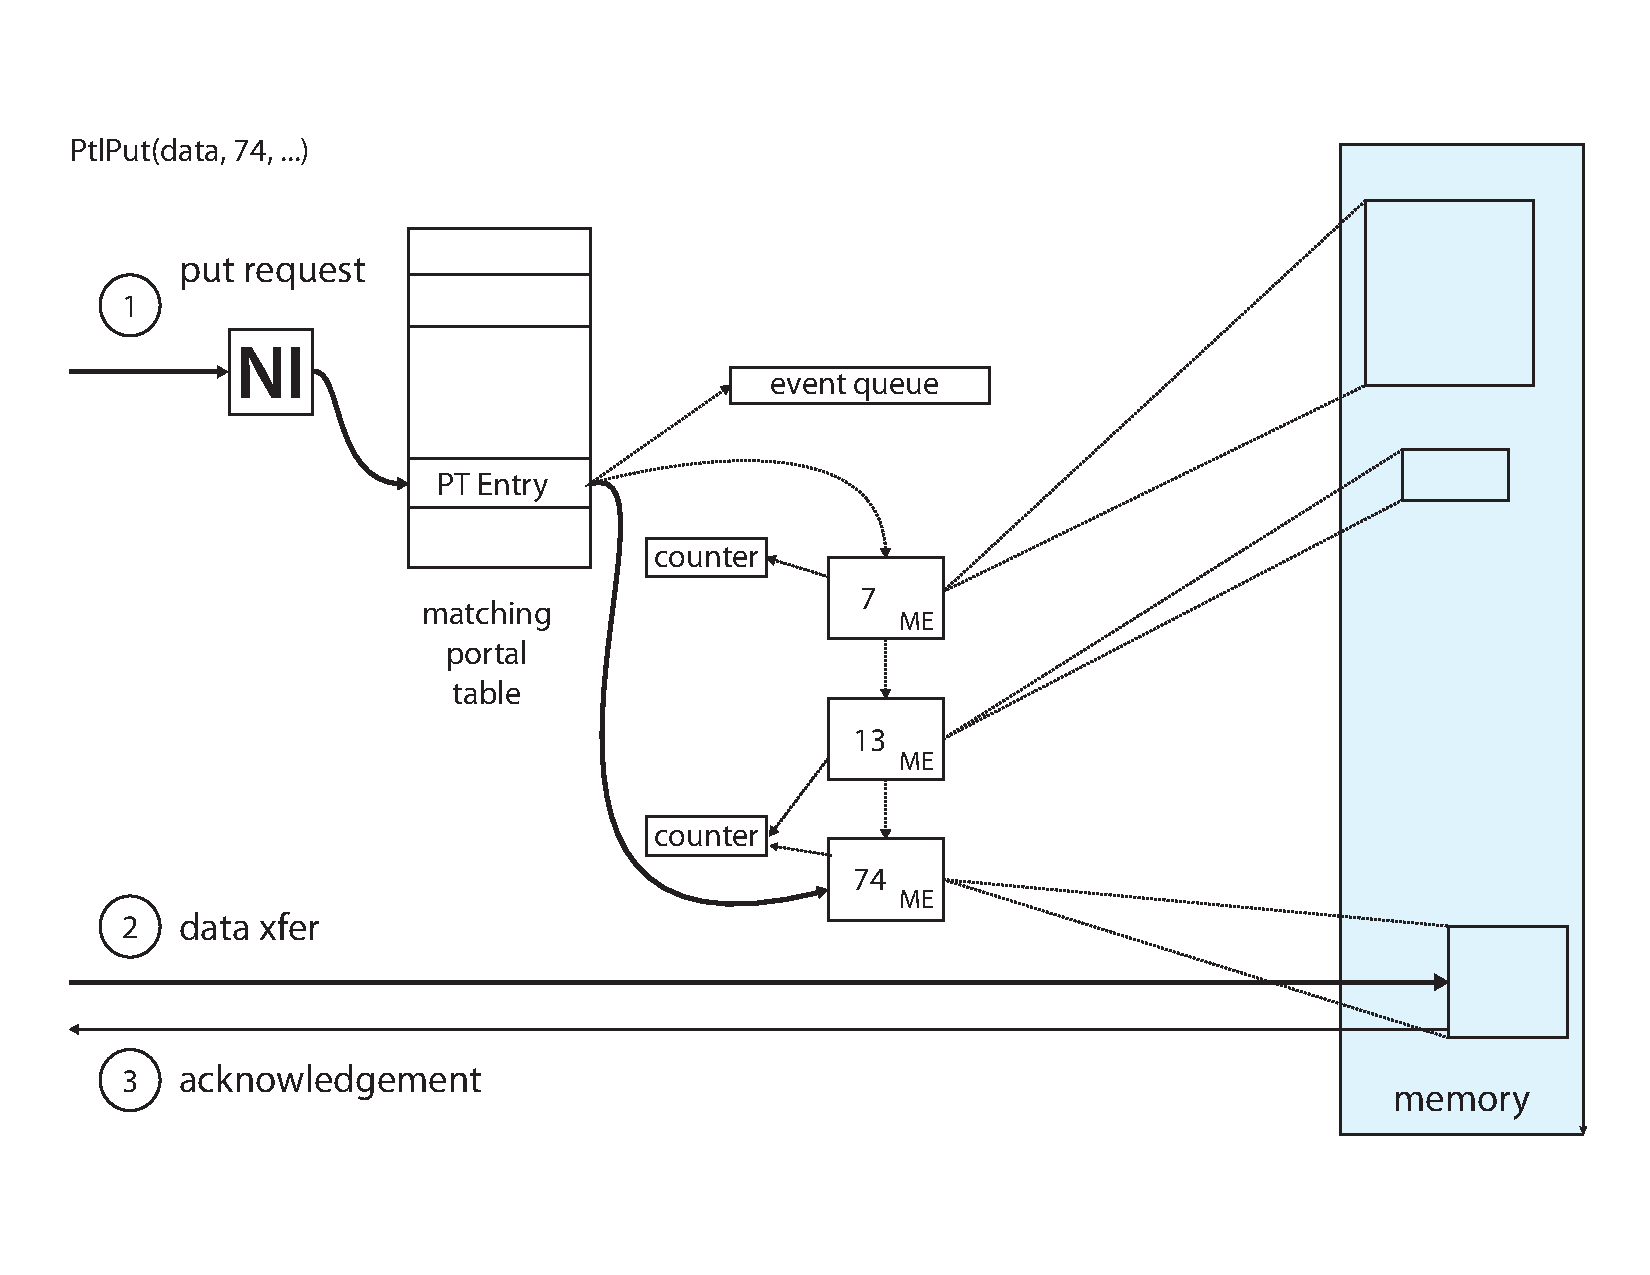
\includegraphics[width=3in]{figs/portals_put}
  \caption{Target-side data abstractions used for a Portals matching interface {\tt put} operation}
  \label{fig:portals_put}
\end{figure}

Portals defines two distinct roles for communication operations. The {\em
  initiator} role is assumed by the process that issues a Portals put, get, or
atomic operation. The {\em target} role is assumed by the process that receives
these operation requests and is responsible for performing the operation or
sending the requested data.

The Portals {\em network interface} (NI) data structure is a per-process
abstraction of a physical network interface and is configured as a
matching or non-matching interface. The NI is associated with both
initiator and target roles. Initiator processes define a {\em memory
  descriptor} (MD) -- a region of memory used for the put/get/atomic
operations as well as ancillary structures used to track communication
events (such as completion) for these operations.

Target processing is expressed with respect to a {\em portal table}. Each NI has one portal 
table containing multiple entries that separate and
classify communication channels between endpoints.  Each {\em portal table
  entry} (PTE) is identified by a unique index into the Portal table. The index
for a specific PTE is a required parameter of all Portals communication
operations. Each PTE maintains a list of memory regions that are valid for
communication operations as well as an event queue, which is used to track
target-side asynchronous notifications.  Some completion information and
notifications may only be visible to the initiator and not the target, or vice
versa.

A PTE using the matching interface maintains a list of match-list entries (ME).
Each ME specifies a set of matching criteria and a memory region associated
with the entry. If the match criteria are satisfied, the communication
operation commences working on corresponding memory region. Matching criteria
consist of multiple parameters, including a 64-bit {\em match bits} field
that must be an exact match in order for an incoming request to to proceed
with the given ME. For example, a process may post an {\tt MPI\_Recv()}, which
creates a new ME on the target PTE with a specific match bits value. Later,
another process would issue an {\tt MPI\_Send()} communication request with
the same match bits that correspond to the previous receive operation.

Portals also provides {\em event queues} and {\em event counters} that can be
used to track data movement in and out of memory regions related to Portals
communication operations. Events and counters also log failure events and
additional information. Counting events are lightweight operations and only
record the success or failure of a given operation. Full events incur more
overhead but contain detailed information about the event and the corresponding
communication operation. Event queues may be associated with an MD
(initiator-side) or a PTE (target-side). 

Event counters are also able to track both initiator and target events. In
contrast to target-side event queues, an event counter may be associated with a
single entry in the match list (an ME), rather that for an entire PTE. PDHT
typically uses lightweight counting events to track successful completions and
full events to track specific failures. Detailed descriptions of how event
queues and counters are used within PDHT is discussed below.

Figure~\ref{fig:portals_put} shows a visual representation of the target-side
structures used in an example {\tt PtlPut()} operation using the matching
interface. We assume that the initiator has issued a {\tt PtlPut()} operation
with some data, a PTE index and the match bits set to 74. Upon receiving the
request, the target process searches the match list for the given PTE until a
74 is found or the end of the list is reached. Once a match has been found the
payload data of the {\tt PtlPut} is copied into the memory region associated
with the ME. The completion of this operation may cause an event to be appended
to the PTE event queue or the ME success counter to be incremented. 
Lastly, an acknowledgement message is sent back to the initiator, possibly
generating another full or counting event associated with the MD that
was used to initiate the {\tt PtlPut} operation. Note that the match list is 
searched in sequential order, preserving message-ordering semantics
typically required by MPI implementations.

In a two-sided model, a send request may arrive at the target prior to the
receive being posted. In addition to the main (priority) match list, Portals
maintains a secondary overflow match list for unexpected messages.  The
overflow list is searched automatically if a matching entry is not found on the
priority match list. The overflow list may also be searched explicitly by
the target-side process (e.g. to match an earlier send to a posted receive).


\subsection{PDHT Implementation}

% serial vs. parallel approaches
Hash tables and key/value stores can be implemented with a myriad of different
techniques but are traditionally implemented sequentially as an array of
pointers to objects.  Parallel implementations typically distribute entries
across nodes. In contrast to sequential versions, the distributed store must
hold the entire value object, rather than just holding a reference to the value
object (to avoid another communication).

% parallel programming model
%  - key/value pairs
%  - object can be located anywhere distributed memory, governed
%     solely by hash function
%  - hash function maps key -> rank/offset tuple
%  - two primary operations put/get
%     - if put yields a collision, then object is placed in next
%        available bucket
%     - get returns object, probing as necessary


Our implementation of the PGLAS data model, PDHT, provides a distributed
key/value store that is accessed using asynchronous one-sided {\em insert,
  read, write,} and {\em atomic update} operations. PDHT uses a traditional
hash function\cite{cityhash} to map an arbitrary user-supplied key to a process
rank and 64-bit hash value. Each key is mapped to a deterministic physical
location within the distributed key/value store.

A PDHT storage structure is represented as a distributed array of objects, with
partitions on all processes. Upon the creation of a new PDHT store, two portal
table entries (PTEs) are allocated. The first PTE is used as the {\em pending}
match list, which is used solely for insert operations.  The second PTE is used
for the {\em active} match list, and is used for all other operations. 

The pending match list is pre-populated with a number of entries that are
configured to match any incoming communication requests (i.e. wildcard
entries). Each match list entry (ME) in the pending list is mapped to a
distinct memory region located in the local portion of the distributed object
array. All MEs on the pending match list are marked as use-once and are
automatically removed from the list after being written to. In contrast, MEs on
the active list may either be marked as use-once or persistent, depending on
the needs of the application.

Every live element in the key/value store has a corresponding active match list
entry. The ME has a reference to the location in the distributed object array
and uses the 64-bit hash value produced by the hash function as the matching
value, ({\em match bits}), in the match list. By using the hashed value of the
key for the match bits field in the ME, the lookup and communication
corresponding to the read operation can be performed entirely by the Portals
implementation.

% adding new entries

% data access

% optimizations
%   - 
%  - fence
%  - other features
%    - atomic counter
%    - barrier/reduce/all-reduce/broadcast
%
%- challenges
%  - poll elimination with triggered updates
%  - matchlist length
%    - multiple portal table entries
%    - Portals 4 unordered matching

% HERE
 
%  - migration from pending to active

\subsection{Inserting Objects}

To insert a new element into the hash table, the process first hashes the key,
yielding both the target processor rank and the 64-bit match bits field used for
the value. Local insertions can be handled as a special-case, by copying the entry
into an available region in the table on the local process and appending a
match list entry onto the active PTE with the match bits set to the value
returned by the hash function. In this case, the local process acts as both 
the initiator and target processes.

If the key hashes to a remote process, the initiator process performs a
one-sided Portals put operation onto the pending PTE of the target rank. This
consumes a wildcard entry on the match list. This process is demonstrated in
Figure \ref{fig:put}. The initial state is shown in Fig. \ref{fig:put}a, with
wildcard entries on the pending match list and available key/value pairs on the
active match list. After the put operation completes, the hashed key match bits
are set on the consumed wildcard ME ($K_4$) and the value data ($V_4$) is
stored into the memory region defined by the match list entry, as can bee seen
in Fig. \ref{fig:put}b.

The value object data is communicated and stored into the memory region defined
by the match list entry. As seen in Figure \ref{fig:put}b, the table entry
resides on the owner process, but the match-list entry is still resident on the
pending match list, rather than the active one. To complete the put operation,
the inserted entry must have a corresponding entry on the active match list,
with the match bits set to the hashed key string. Since the insert operation
consumed a wildcard entry on the pending PTE, it must also be replaced with a
new empty ME.

The final state, represented in Fig. \ref{fig:put}c, shows that the $K_4$ entry
has been appended to the active match list and is available to be accessed by
other processes. Entries are only accessible once they have been appended to
the active match list. The insert operation returns on the initiator side once
it receives an acknowledgement that the target has placed the new entry onto
the pending match list. 

A dedicated progress thread monitors the event queue on
the pending match list and handles the migration of the entry from the pending
list to the active list. The progress thread blocks on the event queue
corresponding to the pending PTE and is notified by Portals whenever a new
insert request arrives. The progress thread replenishes the consumed wildcard
ME on the pending list and appends a new ME to the active match list with the
appropriate match bits set, as can be seen in Fig. \ref{fig:put}c. Any
subsequent data access operations will match against the entry in the active
list.

\begin{figure*}
  \centering
  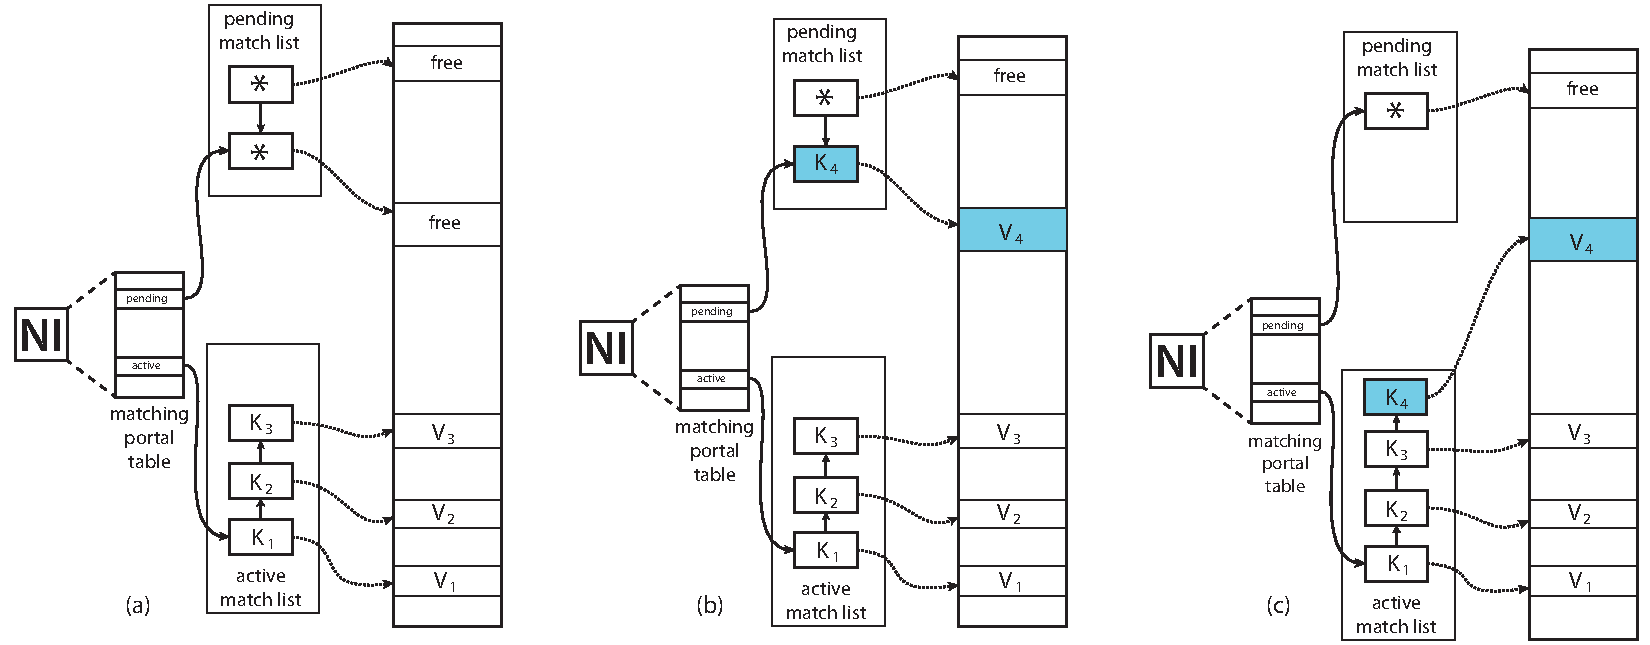
\includegraphics[width=0.85\linewidth]{figs/put}
  \caption{Sequence of target-side actions performed during a \pdht~{\tt insert()} operation.}
  \label{fig:put}
\end{figure*}

% flow control
It is possible for insert operations to outpace the progress thread's ability
to replenish entries on the pending match list. Ideally, the pending match list
size should be large enough to buffer incoming requests, but not as large as
the active lists. PDHT implements a flow control protocol using the Portals
flow control primitives and event notifications to pause insert operations
until there there are valid wildcard entries on the pending match list.
Invoking flow control does incur overhead and may cause multiple communication
attempts. While this increases the time to insert a new entry under a flow
control scenario, it avoids the application programmer burden of selecting an
optimal pending queue size.

\subsection{Accessing Objects}

In contrast to the complexity of adding new items to the PDHT, other
operations, such as reading or updating existing entries, are straightforward.
PDHT supports get, update, and atomic update operations on key/value pairs.
When an operation is requested, the key is hashed to yield the rank and match
bits value. The system then simply invokes the corresponding Portals get, put, or
atomic operation on the active match list with the hashed match bits value.
Portals performs the operation and updates an event counter that increments a
success or failure counter. In the case of a failure, PDHT discriminates a "not
found" error from other networking troubles.

Beyond using read/insert/update operations for working on distributed data,
PDHT also provides an interface to iterate over active entries on the local
process. This functionality allows for owner-compute style programming idioms
and allows for communication-free access to global data entities. Remote fetch
or update operations are not synchronized against local iteration. Overlapping
both models is trivial in a read-only phase but may require external
synchronization when mixing models in general.


\subsection{Additional Features}

Because PDHT is built directly atop the Portals interface, normal programming
features such as collective calls are missing. While PDHT can integrate
seamlessly with a higher-level parallel programming framework such as MPI or
UPC, there is no requirement for a PDHT application to use such a system. As a
result, PDHT has also been extended to provide rudimentary collective
operations such as broadcast, reduce, and all-reduce functions for a limited
set of common datatypes.

PDHT also provides barrier and fence operations for synchronizing processes.
The barrier operation works in the conventional sense, blocking all processes
until the barrier is reached. The fence blocks progress until all outstanding
communication events invoked prior the fence have been completed on the target
process. The PDHT fence operation is implemented as a collective call, which
iteratively compares the number of outstanding communication operations against
the number of completed operations -- the fence terminates when the values
match. 

The runtime also supports global, atomic counters. These counters are typically
used for coarse-grained dynamic load balancing. Global counters are implemented
with lightweight Portals atomic operations. The runtime allocates two
additional Portal table entries (PTEs) to support the collective,
synchronization, and counter operations. 

\subsection{Performance Improvements}
\label{sec:ptl-ext}

\subsubsection{Progress Thread Elimination}
A progress thread is a viable
approach for handling insertion requests but requires target-side processing
by both Portals and PDHT. Portals provides an experimental feature that allows
for a triggered match list append operation to occur when an event counter
exceeds a specified threshold value. We can eliminate the progress thread
altogether by utilizing these {\em triggered append} operations. In this
approach, every PDHT key/value match list and table entry is associated with a
Portals event counter, initially zero.  When the wildcard MEs are created on
the pending list, triggered append operations are also setup to trigger when
the wildcard ME is written to. The responsibility for moving key/value pairs
from the pending list over to the active list is delegated to the Portals layer
(which may be supported with hardware), rather than a separate user-level
progress thread. 

One issue with this approach is that Portals requires the match bits for the
appended entry to be specified at setup time, rather than when the trigger is
executed. Within PDHT, the trigger is set when the wildcard entry is added to
the pending match list, but the active ME's match bits are unknown until a new
entry is placed via a {\tt PtlPut()} on the pending list. This issue does not
impact the current reference implementations of either PDHT or Portals. These
issues could be resolved with alternative Portals implementations under the
current triggered operation semantics by ``chaining'' multiple triggered
operations. Ideally, this additional functionality and semantics should be
incorporated into the Portals specification, in order to ensure that these
programming models are portable across Portals implementations.

\subsubsection{Unordered Matching}

PDHT is able to provide efficient get
operations by having an ME for every entry in the PDHT key/value store. This
design results in match lists that may contain many thousands of entries. When
a get operation is issued, the target side must search the match list for a
matching entry and return the value object associated with the requested key. A
significant challenge to implementing a large-scale key/value store on top of
this approach is that the match list is conventionally implemented as a
linked-list, which much be searched upon any message request. If a process is
hosting a large number of key/value entries, searching this list may be
prohibitively expensive. Traditional uses of the matching interface, such as
implementing MPI message matching, would rarely see match list lengths on the
scale as may be used in PDHT (one per element) \cite{flajslik:16}.

Indeed, initial results showed that match list length had a critical impact on
the access times within PDHT~\cite{comhpc16}. Our first approach to deal with
this issue was to adapt the hash function to map a logical key to a tuple
including the rank, match bits, and a new PTE index value. The PDHT
implementation is able to distribute key/value objects over multiple Portal
table entries. Instead of a single entry with a match list containing 10,000
entries, the system could be configured with 10 PTE match lists, each
containing approximately 1,000 entries. While this technique did reduce match
list overhead, search latency was still substantial, especially on small scale
runs, or with very large datasets.

When used in message-passing libraries, the matching procedure must preserve
the ordering of posted communication operations -- a behavior that is easily
captured with a linked list. However, under the PGLAS approach, no ordering
constraint exists and sequentially searching a linked list unnecessarily slows
performance.

\sloppypar
We have therefore proposed the inclusion of an unordered matching feature on the Portals matching interface
and the corresponding patches has been merged into the Portals reference implementation.
We implemented this extension by adding a {\tt PTL\_PT\_MATCH\_UNORDERED} option that is
specified when creating a new PTE. When the unordered matching option is set,
the match list append operation stores a reference to the ME in a lightweight
hash table~\cite{uthash}.  The search process is also amended to circumvent a
list traversal by first checking the hash table for a matching entry. This
results in much improved performance with respect to the initial
implementation.

\subsubsection{Local Match List Searching}

Initially, all accesses to distributed value objects were made using {\tt
  PtlGet()} operations. The Portals reference implementation makes no
distinction between local and remote data, which adds substantial overhead for
operations on local data.  

Every Portals matching PTE contains two message match lists -- the unexpected
list and priority list. In two-sided communication, such as MPI, an 
{\tt MPI\_Send()} may arrive before the {\tt MPI\_Recv()} is posted. Portals
exposes API to search the unexpected message list to match the send/recv 
messages. A similar approach, but to the priority list (i.e. the active match
list) could be used to improve access for value objects local to the requesting
process.

We added a new priority match list search call to the Portals API and adapted
the existing code in Portals to provide this functionality. When the new search
function is called, an event is generated containing a pointer to the value
object if found, or a failure event otherwise. PDHT get and update operations
check the rank component of the tuple returned by the hash function. When the
object's rank matches the local process, PDHT calls the search function for
local entries rather than calling {\tt PtlGet()} or {\tt PtlPut()}. This
optimization led to a dramatic improvement in access to local data.

\subsection{Hash Collisions} 

A hash collision occurs when multiple keys map to an identical rank/match bits
pair. By default, PDHT detects collisions by comparing the requested key value
against the key of the retrieved object and reporting the condition to the
application. PDHT can also handle collisions transparently within the system by reserving
a small number of match bits to use as alias identifiers and probing multiple
aliases on the requested key when a collision is detected. However, we have
observed that many applications can provide a hash function that is
collision-free.

In traditional hash tables, a hashed key, $K$, is used with modular arithmetic
to select a location in an array of elements of size $N$. The hash function
gives a mapping between $K \rightarrow N$ elements.  If the size of the key
space, $|K|$, is much larger than $N$, the likelihood of collisions increases.
Conventional approaches store a list of objects within each array entry
(chaining) to limit the overhead of collisions.

While PDHT also uses an array to hold the collection of hash table entries, the
indexing into this array is performed indirectly, by Portals. At
initialization, match list entries map to specific table entries. While each
table may be of size $N$, each of the $N$ entries is indexed by the Portals
match bits value, using a hash function that maps from $K \rightarrow 2^{64}$.
Compared to traditional implementations, $N \ll 2^{64}$, which has the impact
of dramatically lowering the probability of a collision, given a reasonable
hash function.


% get operation
%  - run hash
%  - issue PtlGet from active list
%  - check for collision



%  - custom hash functions 
%  - 64-bit hash space, rather than array bucket
%      - detach key -> array size dependency
%      - lower collision rates

% other operations
%  - iteration
%  - non-blocking / bundled puts/gets
%  - interoperability


%%% Local Variables: 
%%% mode: latex
%%% TeX-master: "paper"
%%% End: 
